\documentclass[aspectratio=169,xcolor=table]{beamer}
\usepackage{algorithm}
\usepackage{algpseudocode}
\usepackage[utf8]{inputenc}
\usepackage[T1]{fontenc}
\usepackage{lipsum, lmodern}
\usepackage{csquotes}
\usepackage{xcolor}
\usepackage[portuguese]{babel}

% ------------------------------------------------
% Tema do Beamer (exemplo de um tema customizado)
% ------------------------------------------------
\usetheme{DCC} % <-- Ajuste conforme seu tema ou estilo

\graphicspath{{imgs/}{../resultados/}}
\graphicspath{{imgs/}{../Figuras/}}

\author[Magalhães, Leahy, Felipe]{%
  \textbf{Antoniel Magalhães} \\
  \textbf{João Leahy } \\
  \textbf{Luis Felipe}
}
\title{Problema de Colocação Ótima de Câmeras de Segurança}
\institute{Universidade Federal da Bahia \\ Instituto de Computação}
\date{\today}

\begin{document}

%-------------------------------------------------
%  SLIDE DE TÍTULO
%-------------------------------------------------
\begin{frame}[plain,noframenumbering]
    \titlepage
\end{frame}

%-------------------------------------------------
%  SLIDE DE AGENDA
%-------------------------------------------------
\begin{frame}{Agenda}
    \tableofcontents
\end{frame}

%=================================================
\section{Introdução}
%=================================================
\begin{frame}{Introdução}
    \begin{itemize}
        \item \textbf{Contextualização e Motivação:}
        \begin{itemize}
            \item Aplicação de Teoria dos Grafos em problemas de segurança.
            \item Cenário urbano: bairro de Ondina (Salvador).
        \end{itemize}
        \item \textbf{Justificativa:}
        \begin{itemize}
            \item Modelagem de problemas de vigilância como \emph{Cobertura de Vértices}.
            \item Permite explorar algoritmos gulosos, programação dinâmica e heurísticas.
        \end{itemize}
        \item \textbf{Objetivo Geral:}
        \begin{itemize}
            \item Encontrar o menor conjunto de locais para instalação de câmeras que cubra todas as áreas de interesse.
        \end{itemize}
    \end{itemize}
\end{frame}

%=================================================
\section{Grafo de Ondina}
%=================================================
\begin{frame}{Grafo Bruto de Ondina}
    \begin{figure}
        \centering
        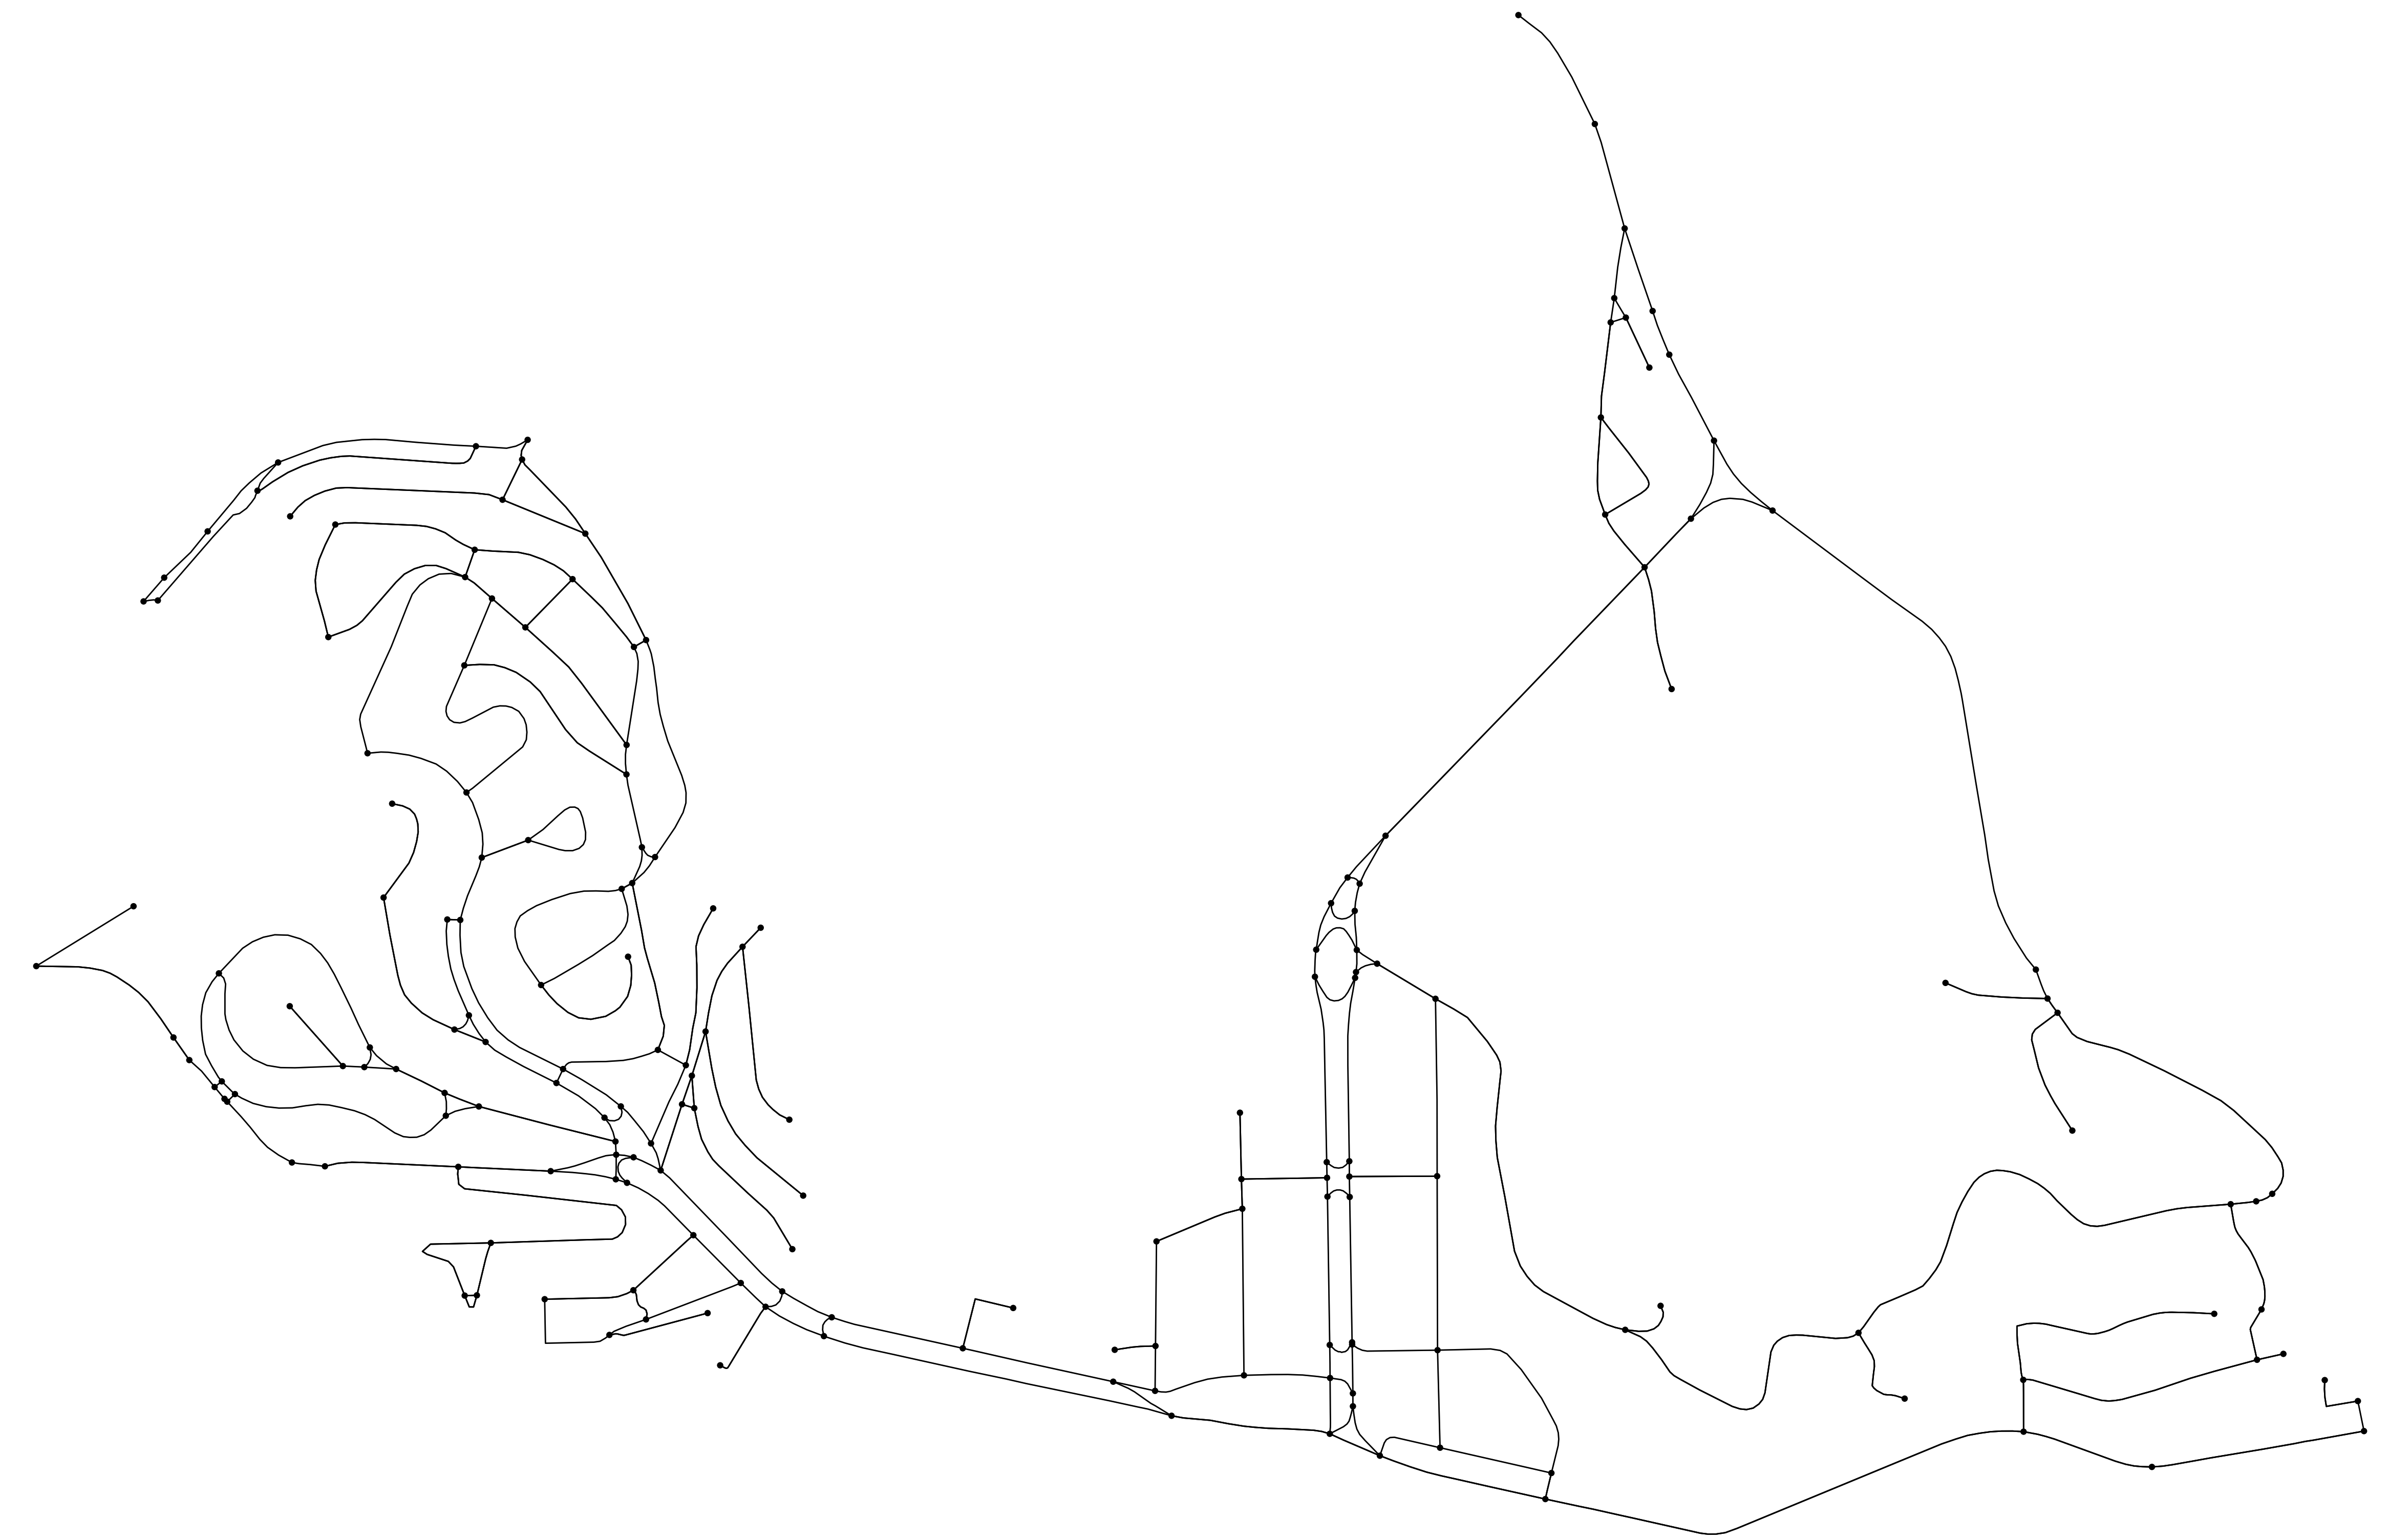
\includegraphics[width=0.8\textwidth]{ondina_grafo_bruto}
    \end{figure}
\end{frame}

\begin{frame}{Grafo Simplificado de Ondina}
    \begin{figure}
        \centering
        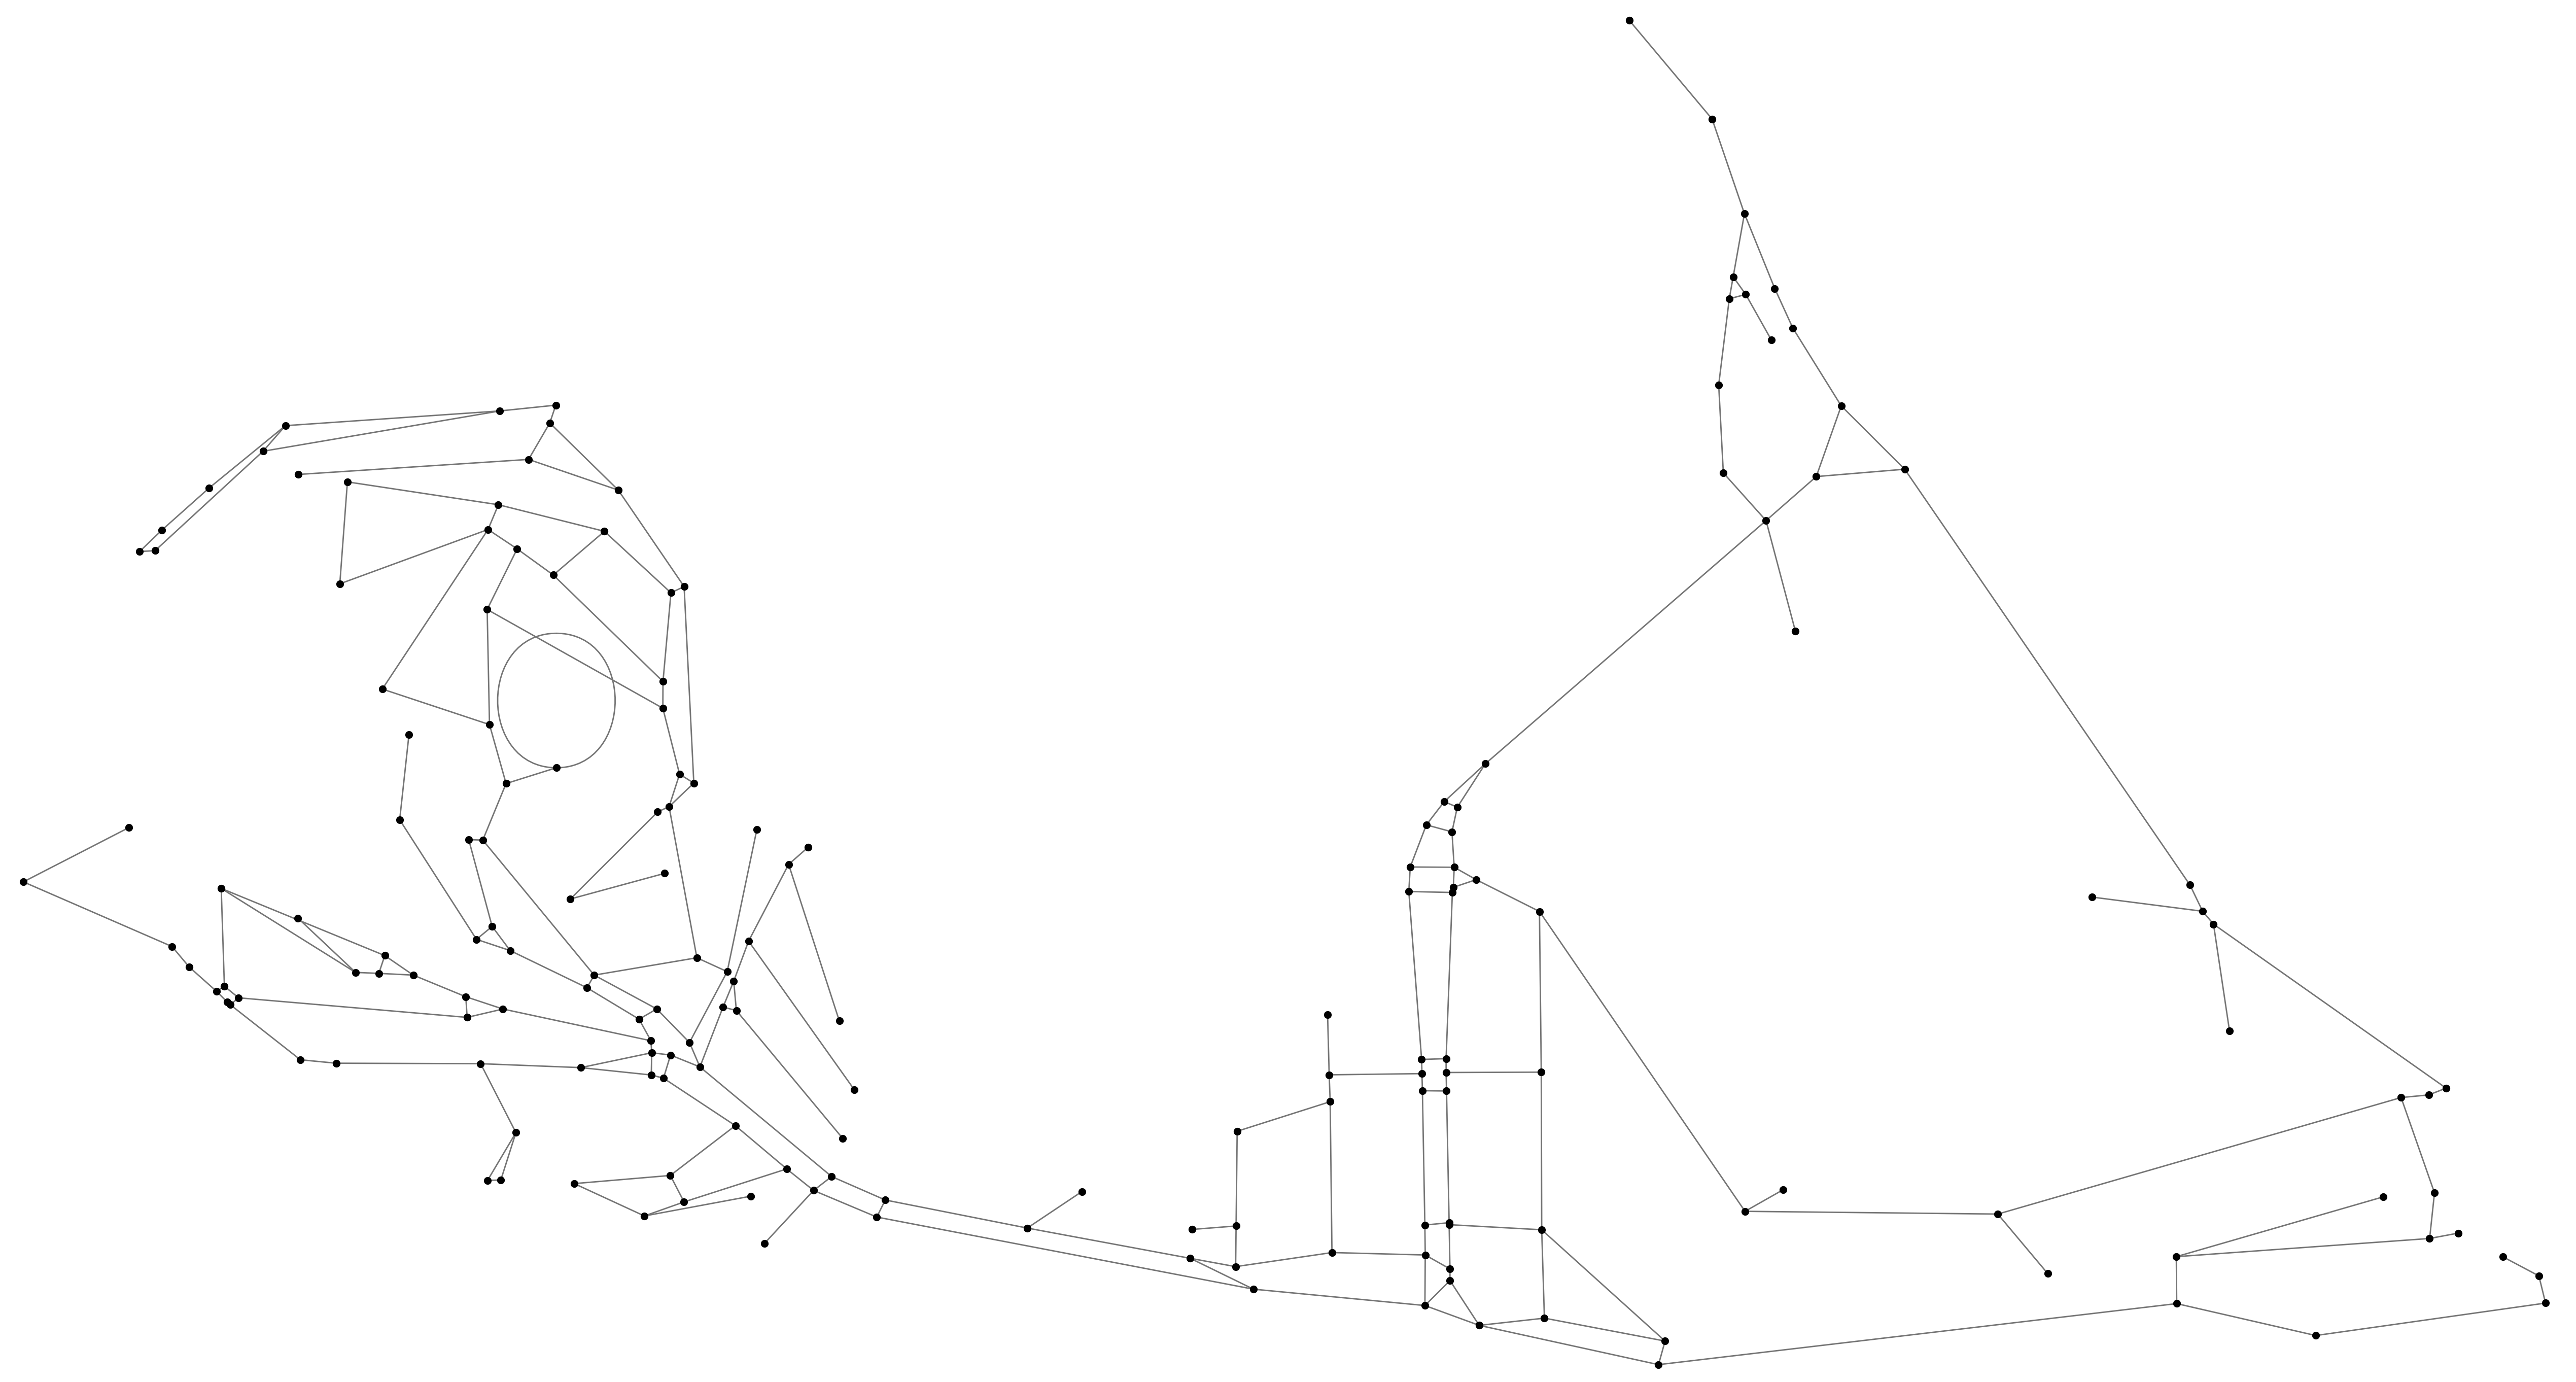
\includegraphics[width=0.8\textwidth]{ondina_grafo_simplificado}
    \end{figure}
\end{frame}

%=================================================
\section{Descrição do Problema}
%=================================================
\begin{frame}{Descrição do Problema}
    \begin{itemize}
        \item \textbf{Formalização:}
        \begin{itemize}
            \item Grafo \(G=(V, E)\): vértices representam locais para câmeras; arestas representam conexões que devem ser monitoradas.
        \end{itemize}
        \item \textbf{Restrições e Função Objetivo:}
        \begin{itemize}
            \item Minimizar número de câmeras (subconjunto de vértices).
            \item Garantir que cada aresta possua ao menos um extremo coberto.
        \end{itemize}
        \item \textbf{Aplicação em Ondina:}
        \begin{itemize}
            \item Extração de dados via OpenStreetMap.
            \item Simplificação das vias em um grafo.
        \end{itemize}
    \end{itemize}
\end{frame}

%=================================================
\section{Solução Algorítmica}
%=================================================
\begin{frame}{Solução Algorítmica}
    \begin{itemize}
        \item \textbf{Cobertura de Vértices:}
        \begin{itemize}
            \item Problema clássico de otimização em grafos.
            \item NP-completo; soluções exatas podem ser inviáveis para grandes instâncias.
        \end{itemize}
        \item \textbf{Abordagem Gulosa (Greedy):}
        \begin{itemize}
            \item Selecionar iterativamente o vértice que cobre o maior número de arestas não cobertas.
            \item Boa eficiência computacional, mas não garante solução ótima em todos os casos.
        \end{itemize}
        \item \textbf{Pseudo-Código (Cobertura Completa):}
        \begin{algorithm}[H]
        \caption{Cobertura de Vértices Gulosa}
        \begin{algorithmic}[1]
        \State $C \gets \emptyset$
        \State $E' \gets E$ \Comment{Conjunto de arestas não cobertas}
        \While{$E' \neq \emptyset$}
            \State Selecione $v \in V$ que incide em mais arestas de $E'$
            \State $C \gets C \cup \{v\}$
            \State Remova as arestas incidentes a $v$ de $E'$
        \EndWhile
        \State \textbf{return} $C$
        \end{algorithmic}
        \end{algorithm}
    \end{itemize}
\end{frame}

%=================================================
\section{Detalhes de Implementação}
%=================================================
\begin{frame}{Detalhes de Implementação}
    \begin{itemize}
        \item \textbf{Ferramentas e Linguagens:}
        \begin{itemize}
            \item Python + NetworkX.
            \item Scripts para extração de dados (OpenStreetMap) e conversão em \texttt{.json}.
        \end{itemize}
        \item \textbf{Estrutura do Projeto (GitHub):}
        \begin{itemize}
            \item \texttt{scripts/}: Implementações das heurísticas, criação do grafo, visualizações.
            \item \texttt{instancias/}: Armazena dados do bairro de Ondina em formato JSON.
            \item \texttt{resultados/}: Saídas dos algoritmos e visualizações.
        \end{itemize}
        \item \textbf{Otimizações:}
        \begin{itemize}
            \item Uso de \texttt{set} para controle de vértices cobertos.
            \item Cálculo incremental das arestas não cobertas.
        \end{itemize}
    \end{itemize}
\end{frame}

%=================================================
\section{Experimentos}
%=================================================
\begin{frame}{Experimentos}
    \begin{itemize}
        \item \textbf{Metodologia:}
        \begin{itemize}
            \item Geração do grafo de Ondina via dados reais (OSM).
            \item Aplicação do Algoritmo Guloso e variações (Cobertura Máxima, p-limitada).
        \end{itemize}
        \item \textbf{Critérios de Avaliação:}
        \begin{itemize}
            \item Taxa de cobertura (arestas ou vértices).
            \item Número de câmeras utilizadas.
            \item Tempo de execução.
        \end{itemize}
    \end{itemize}
\end{frame}

%=================================================
\section{Resultados}
%=================================================
\begin{frame}{Resultados}
    \begin{itemize}
        \item \textbf{Exemplo de Execução em Ondina:}
        \begin{itemize}
            \item Cobertura Completa: 61 câmeras para cobrir 182 vértices.
            \item Cobertura Máxima (p=40): 84\% de cobertura do grafo.
        \end{itemize}
        \item \textbf{Visualização:}
        \begin{itemize}
            \item Gráficos mostram os locais de instalação (pontos vermelhos) e vértices cobertos.
        \end{itemize}
        \item \textbf{Análise:}
        \begin{itemize}
            \item Algoritmos gulosos podem fornecer soluções de boa qualidade em tempo polinomial.
            \item Para restrições orçamentárias, a cobertura máxima parcial pode ser suficiente.
        \end{itemize}
    \end{itemize}
\end{frame}

\begin{frame}{Comparação: Cobertura Completa vs. Máxima}
    \begin{figure}[H]
        \centering
        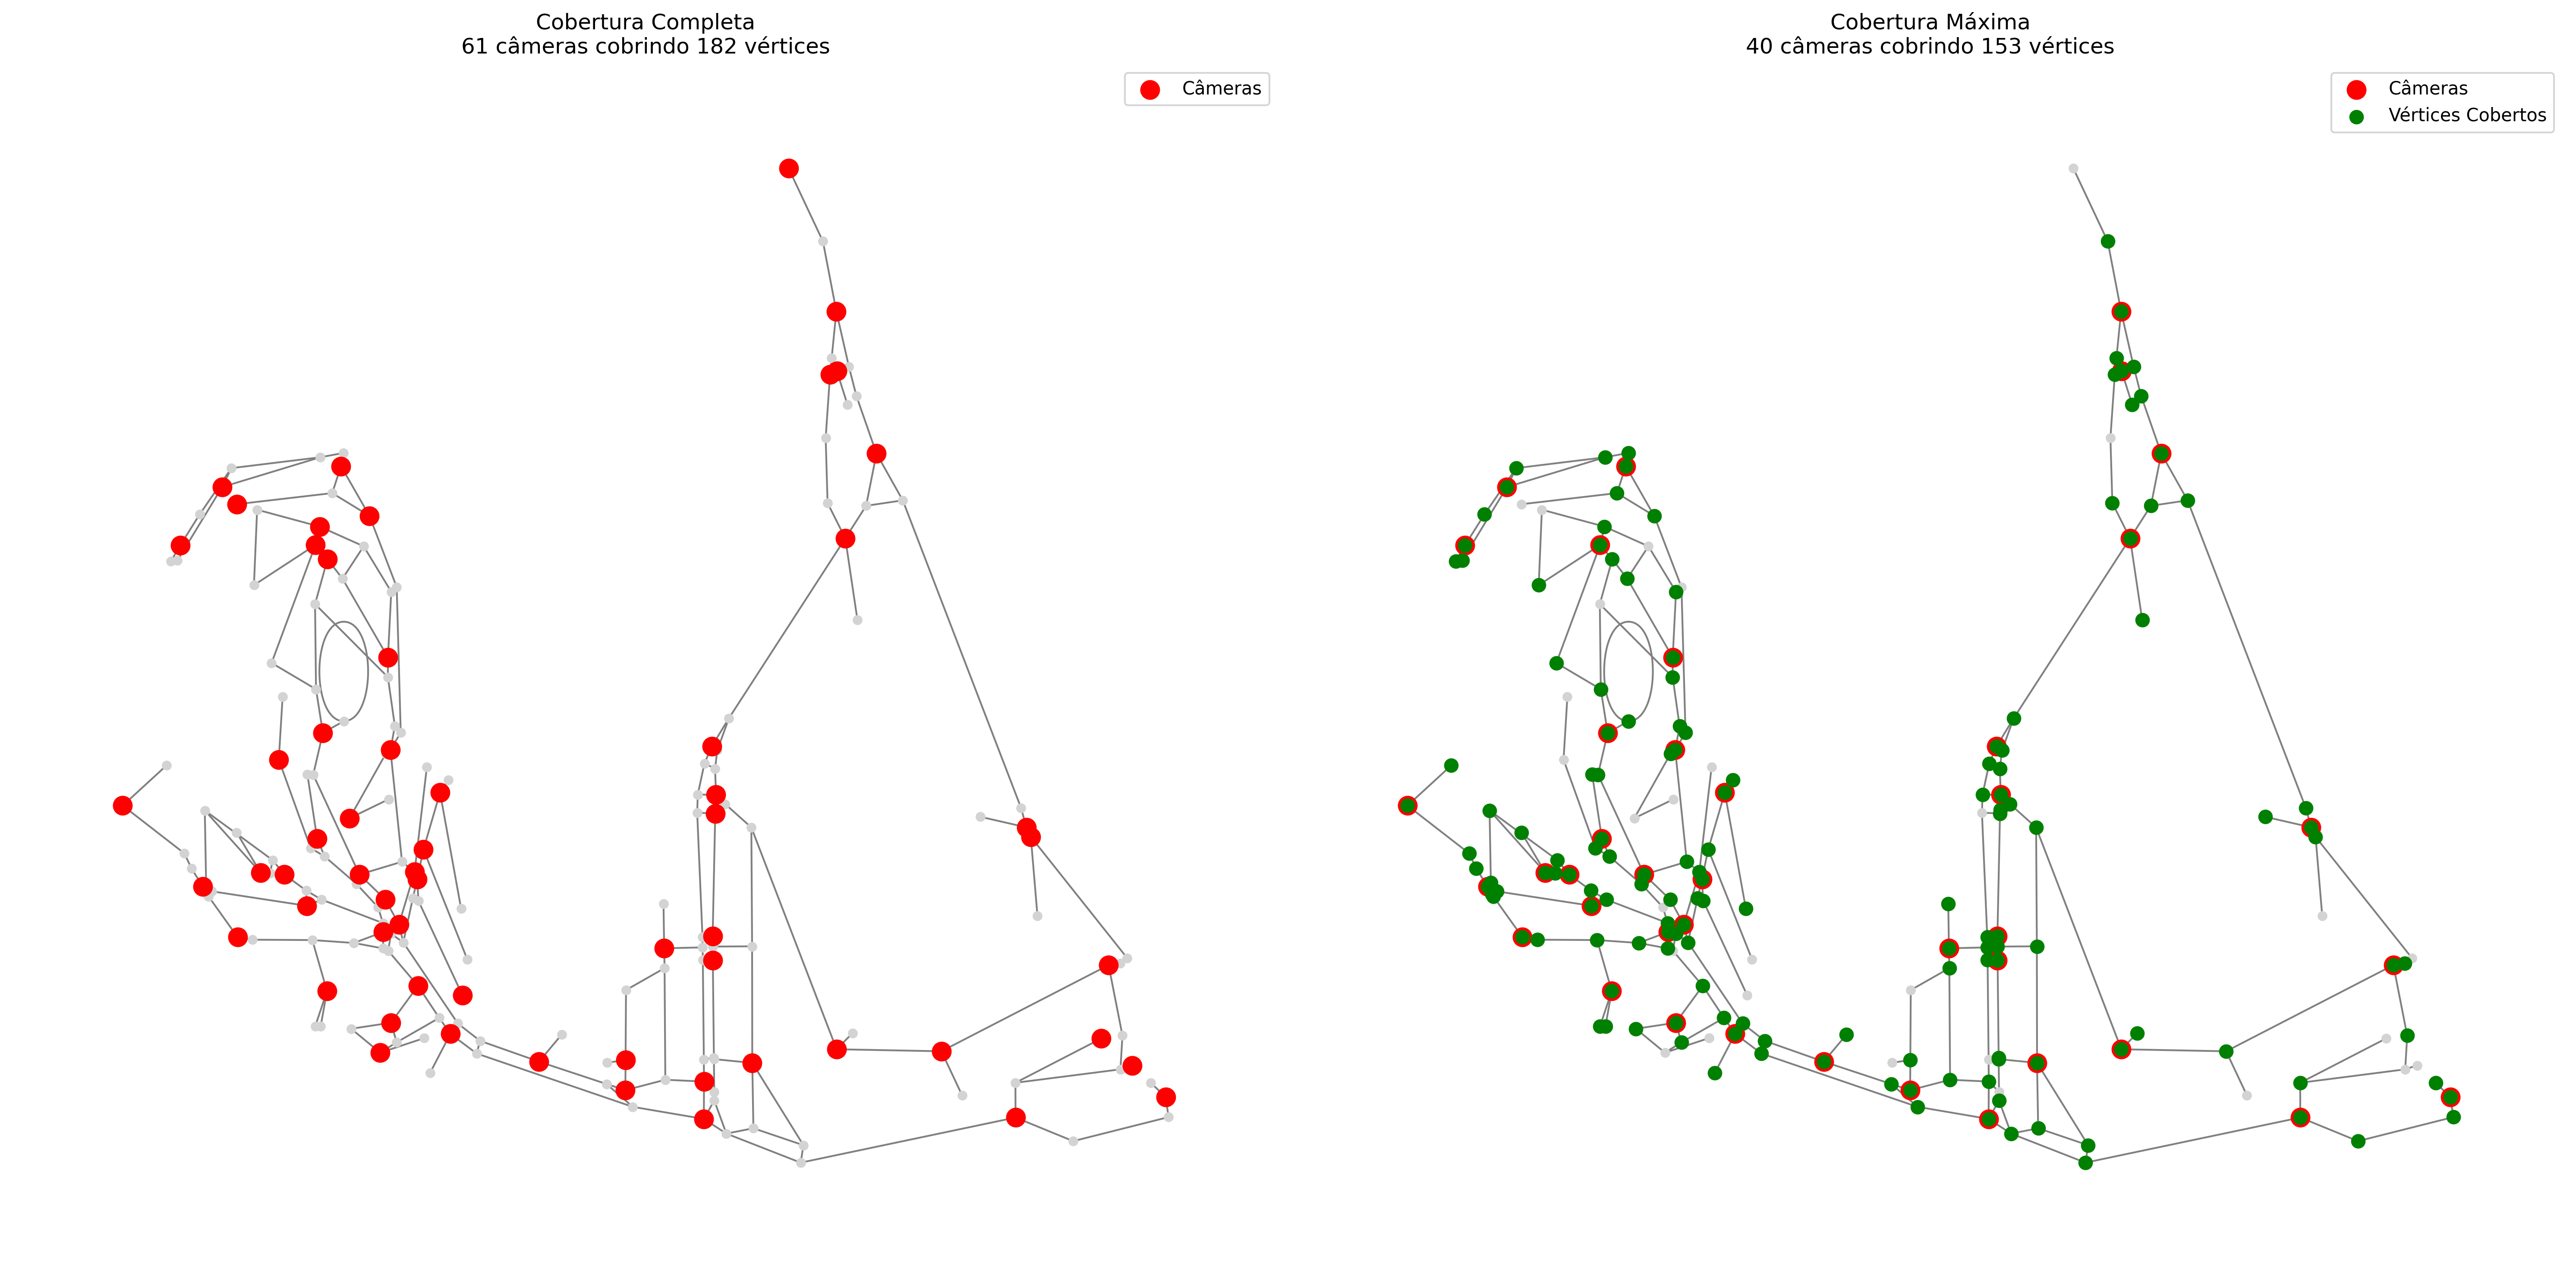
\includegraphics[width=\textwidth]{visualizacao_cobertura}
    \end{figure}
\end{frame}

\begin{frame}{Comparação com Algoritmo Genético}
    \begin{figure}[H]
        \centering
        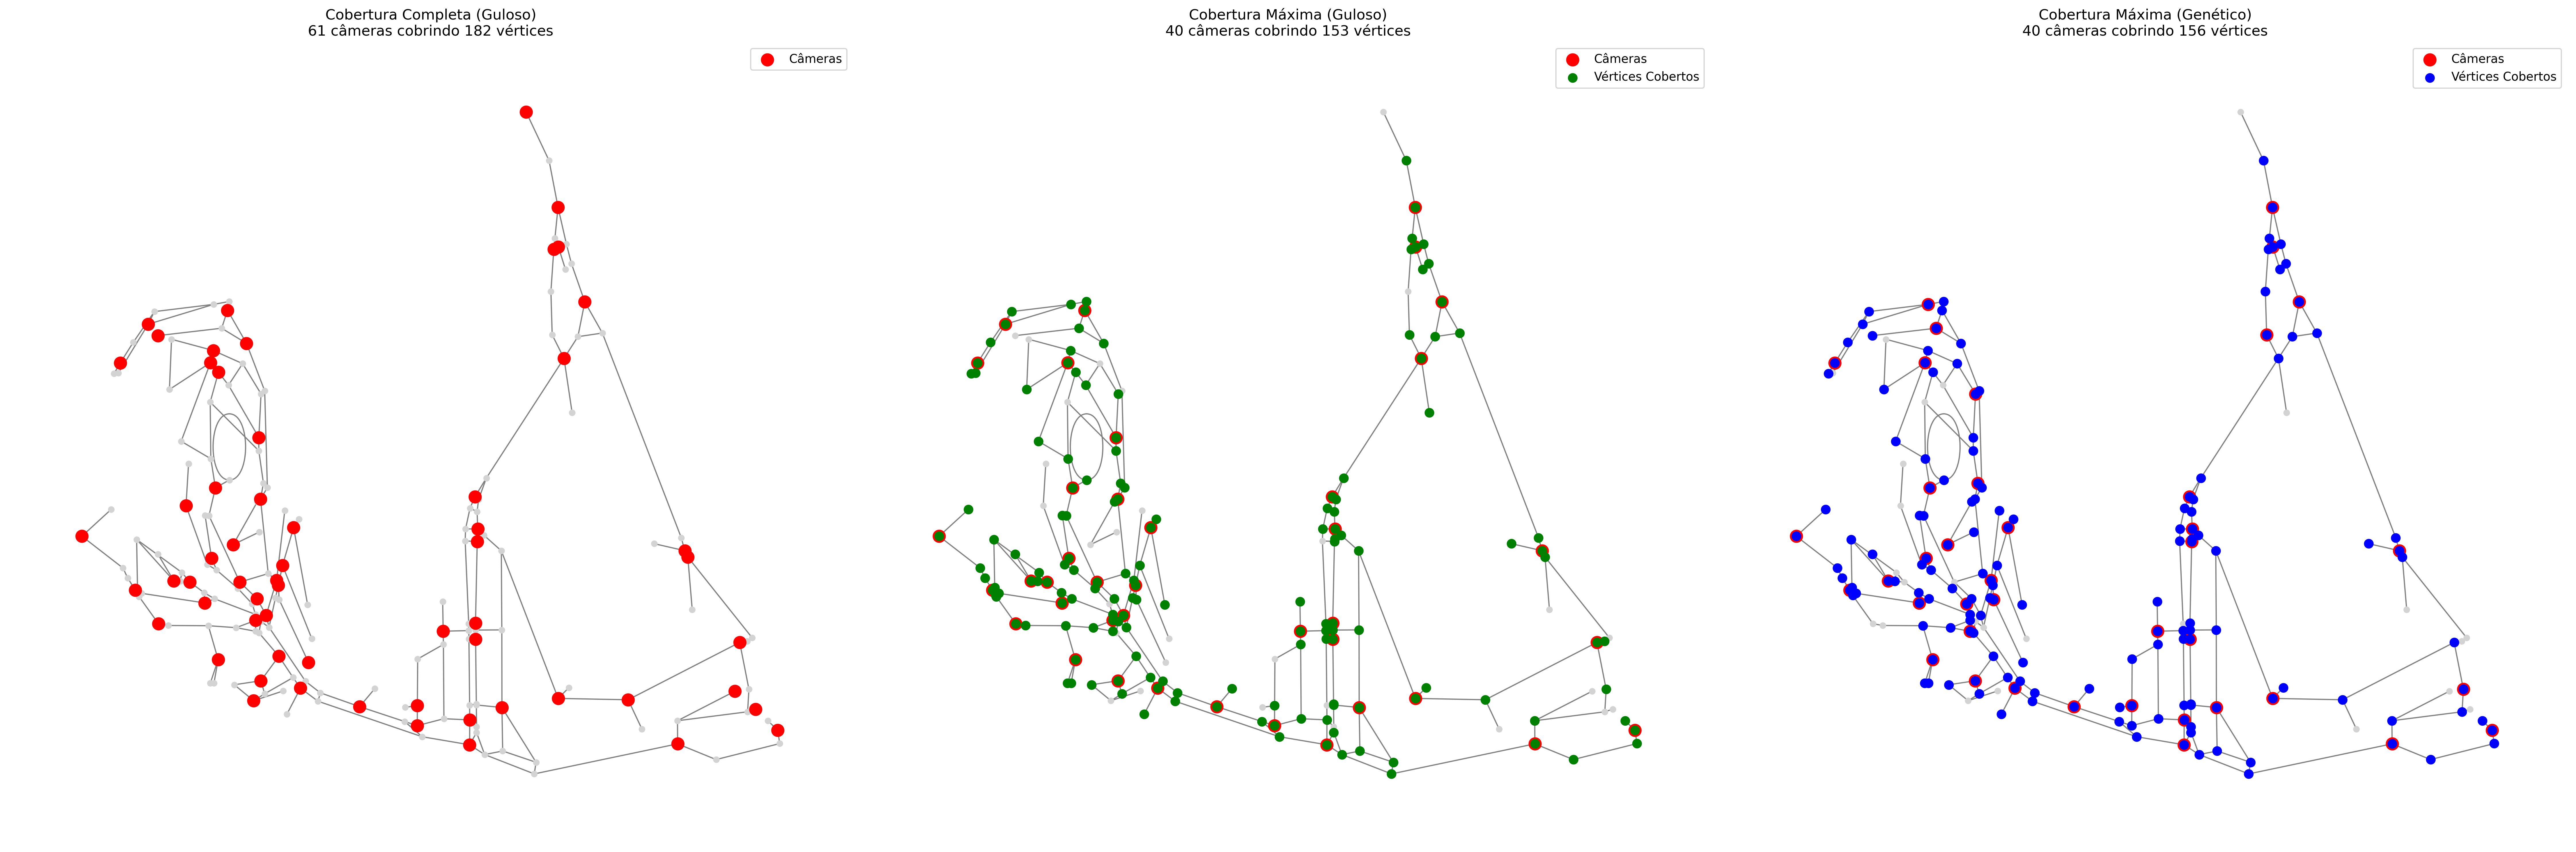
\includegraphics[width=\textwidth]{visualizacao_comparacao}
    \end{figure}
\end{frame}

%=================================================
\section{Conclusão}
%=================================================
\begin{frame}{Conclusão}
    \begin{itemize}
        \item \textbf{Aplicabilidade:}
        \begin{itemize}
            \item Teoria dos Grafos oferece base sólida para problemas de vigilância urbana.
            \item Solução viável para cenários reais de segurança pública.
        \end{itemize}
        \item \textbf{Contribuições:}
        \begin{itemize}
            \item Integração de conceitos de Cobertura de Vértices com dados abertos do OSM.
            \item Comparação entre abordagens gulosas e outras heurísticas (por exemplo, genéticas).
        \end{itemize}
    \end{itemize}
\end{frame}

%=================================================
\section{Referências}
%=================================================
\begin{frame}{Referências}
    \begin{itemize}
        \item Goldbarg, M. e Goldbarg, E. (2012). \emph{Grafos: Conceitos, algoritmos e aplicações}. Elsevier. \cite{goldbarg2012}
        \item Holland, J. H. (1975). \emph{Adaptation in Natural and Artificial Systems}. University of Michigan Press. \cite{Holland1975}
        \item Linden, R. (2006). \emph{Livro algoritmos geneticos}. \cite{Linden2006}
        \item Kleinberg, J. e Tardos, E. (2006). \emph{Algorithm Design}. Pearson Education. \cite{kleinberg2006algorithm}
        \item Repositório do Projeto: \url{https://github.com/antoniel/mata53-projeto-final}
    \end{itemize}
\end{frame}

\end{document}